%% =====================================================================
%% Context-Aware Adaptive Perception for Motorcycle-Dominant Mixed Traffic
%% Target : Journal of Real-Time Image Processing (Springer Nature)
%% Class  : sn-jnl.cls, Springer Nature LaTeX template v3.1 (Dec 2024)
%% Build  : pdfLaTeX + BibTeX. Overleaf: Menu -> Compiler -> pdfLaTeX.
%%
%% Springer asks for ONE .tex file (no \input) with figures as separate
%% files, so the whole manuscript lives here.
%% Every number comes from experiments/ in the CAAP repository; the
%% comment above each table or figure names its evidence file.
%% Before submission, search for "\todo": every hit is an open item and
%% prints in red.
%% =====================================================================
\documentclass[pdflatex,sn-mathphys-num]{sn-jnl}

\usepackage{graphicx}%
\usepackage{multirow}%
\usepackage{amsmath,amssymb,amsfonts}%
\usepackage{amsthm}%
\usepackage{mathrsfs}%
\usepackage[title]{appendix}%
\usepackage{xcolor}%
\usepackage{textcomp}%
\usepackage{manyfoot}%
\usepackage{booktabs}%
\usepackage{algorithm}%
\usepackage{algorithmicx}%
\usepackage{algpseudocode}%
\usepackage{listings}%
\usepackage{tikz}%
\usetikzlibrary{arrows.meta,positioning,calc}%

\theoremstyle{thmstyleone}%
\newtheorem{proposition}{Proposition}%

\raggedbottom

%% Draft marker. Every \todo must be resolved before submission.
\newcommand{\todo}[1]{\textcolor{red}{[TODO: #1]}}

%% =====================================================================
%% DIEN EMAIL TAI DAY -- FILL IN THE E-MAIL ADDRESSES HERE
%% Replace each \textcolor{red}{...} with the plain address, e.g.
%%   \newcommand{\emailNghia}{name@st.ueh.edu.vn}
%% =====================================================================
\newcommand{\emailNghia}{\textcolor{red}{[email Le Trong Nghia]}}
\newcommand{\emailNam}{\textcolor{red}{[email Nguyen Viet Nam]}}
\newcommand{\emailHieu}{\textcolor{red}{[email Ho Minh Hieu]}}
\newcommand{\emailLanh}{\textcolor{red}{[email Vo Xuan Lanh]}}
\newcommand{\emailBao}{\textcolor{red}{[email Nguyen Thien Bao]}}

\begin{document}

\title[Adaptive Perception for Motorcycle-Dominant Traffic]{Context-Aware
Adaptive Perception for Motorcycle-Dominant Mixed Traffic: Class-Conditioned
Motion Modeling and Real-Time Feasibility on Commodity CPUs}

%% Names are ASCII so that pdfLaTeX needs no Vietnamese font encoding;
%% enter the names with diacritics in the journal's submission system.
%% \fnm = given names, \sur = family name (used for indexing).
%% All authors share affiliation [1]; if someone has a different one,
%% add \affil[2]{...} below and change that author's [1] to [2].
\author[1]{\fnm{Trong Nghia} \sur{Le}}\email{\emailNghia}

\author[1]{\fnm{Viet Nam} \sur{Nguyen}}\email{\emailNam}

\author[1]{\fnm{Minh Hieu} \sur{Ho}}\email{\emailHieu}

\author[1]{\fnm{Xuan Lanh} \sur{Vo}}\email{\emailLanh}

\author*[1]{\fnm{Thien Bao} \sur{Nguyen}}\email{\emailBao}

\affil[1]{\orgname{University of Economics Ho Chi Minh City (UEH)},
\orgaddress{\city{Ho Chi Minh City}, \country{Vietnam}}}
%% Add \orgdiv{<faculty / school>} inside \affil if the journal asks for it.

%% JRTIP: 150-250 words, no citations.
%% The last sentence must be revisited once the accuracy of the 448-px
%% operating point is measured (Sect. 6.3).
\abstract{Traffic-surveillance pipelines usually pair a one-stage detector
with a tracker that applies one linear motion model and fixed thresholds to
every object. Both choices are strained in motorcycle-dominant mixed traffic,
where dense weaving fragments identities and a fixed operating point cannot
follow changing conditions. We present a context-aware perception pipeline with
three components: (C1) a context estimator and hysteresis-stabilized controller
that set the tracker's operating point online; (C2) a class-conditioned motion
model that tracks
motorcycles with a constant-turn-rate-and-velocity extended Kalman filter,
re-associates lost tracks inside the filter's innovation ellipse and scales
measurement noise by detection confidence; and (C3) a track reliability score
with separate thresholds for incident alerting and signal-control observations.
On 600 human-annotated rush-hour CCTV frames from Ho Chi Minh City, C2 raises
motorcycle IDF1 from 0.858 to 0.907 and cuts identity switches by
80\% relative to ByteTrack on identical detections. Its components are
super-additive: added to the CTRV filter alone, covariance gating increases
identity switches by 26\%; it helps only together with confidence-scaled noise. Context adaptation did not outperform a calibrated
fixed threshold in the single traffic regime our labels cover, and the
reliability score separated true from false tracks too weakly (ROC AUC 0.609)
to filter usefully after C2; we report both as characterized negative results.
On a CPU, C2 adds 2.8\% to the end-to-end frame time while the detector
takes 91\%; with a detection head instead of the deployed segmentation head,
the pipeline's latency fits a 40~ms budget at 448-pixel input.}

\keywords{Multi-object tracking, Extended Kalman filter, Mixed traffic,
Motorcycles, Context-aware perception, Real-time video analytics}

\maketitle

%% =====================================================================
\section{Introduction}\label{sec:intro}
%% =====================================================================

Road-traffic injuries remain a leading cause of death worldwide, and the burden
falls disproportionately on low- and middle-income countries; in Viet Nam,
motorcycles are the dominant vehicle type and are involved in the majority of
road-traffic deaths~\cite{WHO2023_roadsafety}. Urban intersections are
increasingly covered by fixed CCTV cameras, and two applications motivate
turning that footage into structured perception in real time: incident
alerting, which must not flood operators with false alarms, and adaptive signal
control by multi-agent reinforcement learning~\cite{Chu2020_marltsc,Yu2022_mappo},
which needs complete and temporally consistent observations of the vehicles
approaching each intersection. Both consume the output of the same front end: a
one-stage object detector~\cite{Redmon2016_yolo,Jocher2024_yolo11} followed by a
tracking-by-detection multi-object tracker~\cite{Bewley2016_sort,Zhang2022_bytetrack}.

In motorcycle-dominant mixed traffic this front end fails in two characteristic
ways. The first is \emph{identity fragmentation}. Motorcycles weave through the
gaps between larger vehicles and occlude one another at irregular angles; the
constant-velocity Kalman filter~\cite{Kalman1960} shared by mainstream trackers
coasts along a straight line through an occlusion while the hidden motorcycle
keeps turning, so the reappearing detection falls outside the association region
and receives a new identity. To a signal controller, a fragmented identity is one
vehicle that vanishes and another that appears from nowhere. The second is
\emph{operating-point rigidity}. Confirmation thresholds and track lifetimes are
tuned once, for one regime, yet traffic density, illumination and the share of
spurious tracks change over the day; a setting that suits free-flowing daytime
traffic is wrong for a dense queue or a night scene, and an alerting channel
inherits every spurious track that survives the tracker.

Existing work addresses parts of this problem but not their combination. Recent
trackers strengthen association with appearance
cues~\cite{Wojke2017_deepsort,Du2023_strongsort}, observation-centric
corrections~\cite{Cao2023_ocsort}, camera-motion
compensation~\cite{Aharon2022_botsort,Yi2024_ucmctrack} or learned nonlinear
motion predictors~\cite{Qin2023_motiontrack,Lv2024_diffmot}, yet each applies one
motion model to every object class, and the benchmarks that drive them---crowds
of pedestrians~\cite{Milan2016_mot16,Dendorfer2020_mot20}, dancers and
athletes~\cite{Sun2022_dancetrack,Cui2023_sportsmot}, or road traffic without a
motorcycle class~\cite{Wen2020_uadetrac}---do not exhibit motorcycle weaving.
Kinematic models with an explicit turn rate, such as constant turn rate and
velocity (CTRV), are standard in automotive sensor
fusion~\cite{Schubert2008_ctrv,BarShalom2001_estimation,Lefevre2014_motionsurvey}
but are rarely used in image-plane tracking-by-detection and, to our knowledge,
have not been selected by the detected object class. Context-aware perception,
for its part, adapts to appearance changes such as adverse
weather~\cite{Liu2022_iayolo,Chen2018_dafrcnn} while leaving the tracker's
operating point and motion assumptions fixed.

This paper studies a perception pipeline that adapts to its context along two
axes: per object class, through the motion model, and per traffic regime,
through the operating point. It makes three contributions.
\begin{itemize}
\item \textbf{C1, a context estimator and adaptive parameter controller.} Scalar
context signals computed from the frame and the current track set select the
tracker's confirmation threshold, lost-track buffer and motorcycle motion model
online, with exponential smoothing and hysteresis against oscillation
(Sect.~\ref{sec:c1}).
\item \textbf{C2, a class-conditioned motion model.} Motorcycle tracks are
predicted by a CTRV extended Kalman filter (EKF) inside
ByteTrack~\cite{Zhang2022_bytetrack}, while other classes keep the linear filter.
The EKF's innovation covariance re-opens association for lost motorcycle tracks
that box overlap cannot recover, and its measurement noise is scaled by detection
confidence. We derive the filter, bound its discretization error and
characterize when its state is observable (Sect.~\ref{sec:c2}).
\item \textbf{C3, a dual-task track reliability score.} One score per track,
combining age, detection consistency, motion smoothness, class stability and
detection confidence, is split by two thresholds into a precision-first alerting
branch and a recall-first observation branch (Sect.~\ref{sec:c3}).
\end{itemize}

We evaluate every component against 600 human-annotated frames of rush-hour
footage from Ho Chi Minh City, with identical detections for every
configuration, and we measure the pipeline's cost end to end on a commodity CPU.
C2 is the validated contribution: it raises motorcycle IDF1 from 0.858 to 0.907
and removes 80\% of identity switches relative to ByteTrack, and its parts are
strongly super-additive---covariance gating on its own makes identity
\emph{worse}. C1 and C3 do not improve the tracking metrics on these data; we
report both as characterized negative results and state what evidence would
validate or refute them. The evaluation also yields three methodological
findings that we expect to transfer beyond this pipeline: annotation error in
tracking ground truth is direction-dependent, and over-merged identities inflate
exactly the gap-bridging behavior that a motion model supplies
(Sect.~\ref{subsec:annotation}); proxy metrics computed without ground truth can
be optimized into wrong merges (Sect.~\ref{subsec:proxy}); and on a CPU the
detector, not the tracker, decides real-time feasibility, with the choice of
detection head mattering more than the choice of inference runtime
(Sect.~\ref{sec:realtime}).

The remainder of the paper is organized as follows. Section~\ref{sec:related}
reviews related work and Sect.~\ref{sec:method} details C1--C3.
Section~\ref{sec:setup} describes the data, ground truth and protocol, and
Sect.~\ref{sec:results} reports the results. Section~\ref{sec:realtime} analyzes
computational cost and real-time feasibility, Sect.~\ref{sec:discussion}
discusses methodological lessons and threats to validity, and
Sect.~\ref{sec:conclusion} concludes.

%% =====================================================================
\section{Related work}\label{sec:related}
%% =====================================================================

\subsection{Tracking by detection and motion models}\label{subsec:rw_mot}

Tracking-by-detection pipelines link per-frame detections into trajectories by
predicting each track forward and solving an assignment problem.
SORT~\cite{Bewley2016_sort} combined a constant-velocity Kalman filter with
intersection-over-union (IoU) matching; DeepSORT~\cite{Wojke2017_deepsort} added
appearance descriptors and gated assignments by the Mahalanobis distance under
the filter's covariance; ByteTrack~\cite{Zhang2022_bytetrack} recovered occluded
objects by associating low-score detections in a second stage. Later trackers
refined each part of this loop. OC-SORT~\cite{Cao2023_ocsort} re-updates the
filter from observations after an occlusion to undo the error accumulated while
coasting; BoT-SORT~\cite{Aharon2022_botsort} and
UCMCTrack~\cite{Yi2024_ucmctrack} compensate camera motion, the latter tracking
on the ground plane with a mapped Mahalanobis distance;
StrongSORT~\cite{Du2023_strongsort} adopts the confidence-dependent measurement
noise introduced in GIAOTracker~\cite{Du2021_giaotracker};
Hybrid-SORT~\cite{Yang2024_hybridsort} adds confidence and height cues to the
filter state; Deep OC-SORT~\cite{Maggiolino2023_deepocsort} weighs appearance
adaptively; and FastTracker~\cite{Hashempoor2025_fasttracker} exploits scene
structure to handle occlusion. All of these predict every object with the same
linear motion model.

Nonlinear motion has been addressed mainly by learning.
DanceTrack~\cite{Sun2022_dancetrack} and SportsMOT~\cite{Cui2023_sportsmot}
showed that diverse, fast-changing motion breaks the constant-velocity
assumption, and learned predictors such as MotionTrack~\cite{Qin2023_motiontrack}
and DiffMOT~\cite{Lv2024_diffmot} replace the Kalman prediction with trained
networks. These predictors are class-agnostic and need training trajectories from
the target domain, which for motorcycle traffic are not publicly available
(Sect.~\ref{subsec:rw_mixed}). Model-based alternatives come from vehicle
tracking with range sensors: Schubert et al.~\cite{Schubert2008_ctrv} compared
linear and curvilinear models and found that models with an explicit turn rate,
such as CTRV, track maneuvering vehicles better; interacting-multiple-model
filters~\cite{Blom1988_imm,BarShalom2001_estimation} switch between such models;
and physics-based models form the first tier of motion-prediction
taxonomies~\cite{Lefevre2014_motionsurvey}. C2 brings a CTRV model into
image-plane tracking-by-detection, selects it by detected class and reuses its
covariance for association. Unlike DeepSORT's Mahalanobis gate, which constrains
every assignment, ours applies only to lost tracks of one class and can only add
candidate matches, never override an overlap-based one.
Table~\ref{tab:positioning} summarizes these relations.

%% Positioning table: properties as described in the cited papers.
\begin{table}[t]
\caption{Motion modeling in representative trackers. A check mark records a
design element as described in the cited paper; the comparison is simplified.}
\label{tab:positioning}
\footnotesize
\begin{tabular}{@{}lllcc@{}}
\toprule
Tracker & Motion model & Class-conditioned & Covariance in & Learned \\
        &              & motion model      & association   & motion \\
\midrule
SORT~\cite{Bewley2016_sort}                & linear KF                   & -- & --         & -- \\
DeepSORT~\cite{Wojke2017_deepsort}         & linear KF                   & -- & \checkmark & -- \\
ByteTrack~\cite{Zhang2022_bytetrack}       & linear KF                   & -- & --         & -- \\
OC-SORT~\cite{Cao2023_ocsort}              & linear KF, re-update        & -- & --         & -- \\
StrongSORT~\cite{Du2023_strongsort}        & linear KF, NSA              & -- & \checkmark & -- \\
UCMCTrack~\cite{Yi2024_ucmctrack}          & linear KF, ground plane     & -- & \checkmark & -- \\
Hybrid-SORT~\cite{Yang2024_hybridsort}     & linear KF, extended state   & -- & --         & -- \\
DiffMOT~\cite{Lv2024_diffmot}              & diffusion predictor         & -- & --         & \checkmark \\
Ours (C2)                                  & CTRV-EKF / linear KF        & \checkmark & \checkmark$^{a}$ & -- \\
\botrule
\end{tabular}
\footnotetext[a]{Only for lost motorcycle tracks, as an additional candidate
match (Sect.~\ref{subsec:gate}).}
\end{table}

\subsection{Perception in mixed and motorcycle-dominant traffic}\label{subsec:rw_mixed}

Public tracking benchmarks for road traffic are dominated by cars.
UA-DETRAC~\cite{Wen2020_uadetrac} provides fixed-camera sequences with identity
annotations but labels cars, buses, vans and other vehicles, with no motorcycle
class. Datasets from South and Southeast Asia capture two-wheelers for other
tasks: IDD~\cite{Varma2019_idd} offers driving-view detection and segmentation on
Indian roads, and Siebert and Lin~\cite{Siebert2020_helmet} detect helmet use in
motorcycle traffic. Closest to our setting, Vu et al.~\cite{Vu2025_counting}
detect, track and count vehicles at motorcycle-dominated intersections in Viet
Nam, stabilizing their counts with a modified box reference point and explicit
handling of identity switches; their evaluation targets count accuracy rather
than identity preservation, and their data are not described as public.
TrafficMOT~\cite{Liu2024_trafficmot} targets multi-class tracking in complex
traffic scenes. We found no public fixed-camera benchmark of motorcycle-dominant
traffic with identity annotations over sequences long enough to test
re-association across occlusions, and therefore annotated our own
(Sect.~\ref{subsec:gt}). The class-conditioned design makes this unavoidable: on
data without a motorcycle class, the CTRV branch never executes.

\subsection{Accident detection from traffic video}\label{subsec:rw_accident}

Vision-based accident detection and anticipation have been surveyed
recently~\cite{Fang2024_accidentsurvey,Adewopo2023_review}. Surveillance
datasets such as CADP~\cite{Shah2018_cadp} and dashcam collections such as
D$^2$-City~\cite{Che2019_d2city}, DoTA~\cite{Yao2023_dota} and the dataset of Bao
et al.~\cite{Bao2020_ccd} support clip-level detection, anomaly localization and
anticipation, while tracking-based methods derive accident cues from
trajectories, e.g., abrupt changes of speed and heading~\cite{Ijjina2019_accident}.
Commercial incident-detection systems~\cite{Hikvision_AID} target highway scenes
dominated by cars. Across this line of work the operating point is fixed
offline. How the quality of upstream tracks affects alert precision, and how one
track stream can serve both an alerting channel and a controller with opposite
precision--recall preferences, have received little attention.

\subsection{Context-aware and adaptive perception}\label{subsec:rw_adaptive}

Adaptive perception mostly targets appearance shift: Image-Adaptive
YOLO~\cite{Liu2022_iayolo} learns image-enhancement parameters for adverse
weather, and domain-adaptive detectors~\cite{Chen2018_dafrcnn} align features
across conditions. Within tracking, adaptation is usually local to one detection
or track: confidence-scaled measurement
noise~\cite{Du2021_giaotracker,Du2023_strongsort}, confidence-aware
association~\cite{Yang2024_hybridsort} or adaptive appearance
weighting~\cite{Maggiolino2023_deepocsort}. Selecting tracker hyperparameters
and motion models from measured scene context at run time, as C1 does, and
serving two downstream consumers with opposite error preferences from one scored
track stream, as C3 does, are outside the scope of these methods.

\subsection{Real-time inference on commodity hardware}\label{subsec:rw_realtime}

One-stage detectors~\cite{Redmon2016_yolo} remain the default for real-time
video analytics, with recent members such as
YOLO11~\cite{Jocher2024_yolo11,Khanam2024_yolo11}, YOLOv10~\cite{Wang2024_yolov10}
and RT-DETR~\cite{Zhao2024_rtdetr} trading accuracy against latency. Deployment
commonly exports the network to an inference runtime such as ONNX
Runtime~\cite{ONNXRuntime} or OpenVINO~\cite{OpenVINO}, optionally with integer
quantization~\cite{Jacob2018_quant}. Real-time claims are usually made on GPUs,
whereas many municipal video servers and roadside units have only CPUs; we
therefore report end-to-end CPU latency with the detector included and isolate
what each design choice costs.

%% =====================================================================
\section{Method}\label{sec:method}
%% =====================================================================

\subsection{System overview}\label{subsec:overview}

Figure~\ref{fig:pipeline} shows the pipeline. At frame $t$ the context estimator
(C1) summarizes the traffic state from the frame and from the tracks produced at
$t-1$, and the controller (C1) maps that state to the tracker's operating point.
The detector runs once per frame at a fixed, low confidence floor of $0.1$, so
that low-score boxes remain available to ByteTrack's second association
stage~\cite{Zhang2022_bytetrack}; the adaptive threshold therefore acts on the
tracker, not on the detector. Detections enter a modified ByteTrack in which
motorcycle tracks are predicted by a CTRV-EKF and all other classes by the
original linear filter (C2). The two-stage association is unchanged, except that
lost motorcycle tracks may additionally be matched inside the EKF's innovation
ellipse. Every output track then receives a reliability score (C3), and two
thresholds route tracks to the accident branch and to the observation builder of
a signal controller.

A detection is a tuple $(\mathbf{b},s,\kappa)$ of box
$\mathbf{b}=[x_1,y_1,x_2,y_2]$, confidence $s\in[0,1]$ and class
$\kappa\in\{\textsc{car},\textsc{motorcycle},\textsc{bus},\textsc{truck},\textsc{accident}\}$.
The \textsc{accident} class marks image regions that show a collision; tracks of
that class feed the accident branch (Sect.~\ref{sec:c3}).

%% Pipeline figure, drawn in TikZ (source of paper/figures/fig1_pipeline_overview.tex,
%% with the frame rate corrected to 25 fps and the fifth score term added).
\begin{figure}[t]
\centering
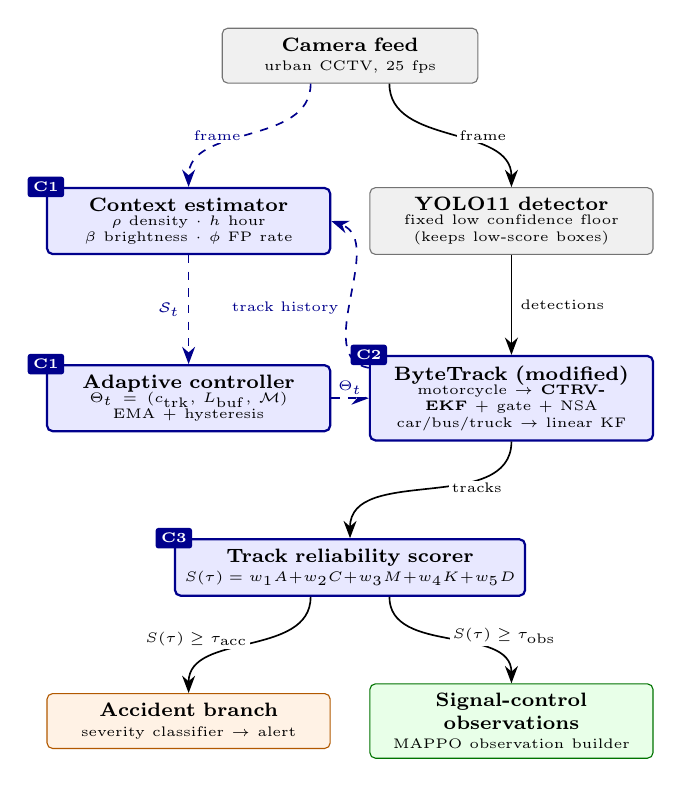
\begin{tikzpicture}[
  font=\scriptsize,
  box/.style={draw=black!55, fill=black!6, rounded corners=2pt,
              align=center, inner sep=3.5pt, text width=3.35cm},
  contrib/.style={box, draw=blue!55!black, fill=blue!9, thick},
  outacc/.style={box, draw=orange!70!black, fill=orange!10},
  outobs/.style={box, draw=green!45!black, fill=green!9},
  tag/.style={fill=blue!55!black, text=white, font=\tiny\bfseries,
              inner sep=2pt, rounded corners=1pt},
  data/.style={-{Stealth[length=2.2mm]}, semithick},
  ctrlarrow/.style={-{Stealth[length=2.2mm]}, semithick, dashed,
                    draw=blue!55!black},
  lbl/.style={font=\tiny, inner sep=1pt, fill=white},
  clbl/.style={lbl, text=blue!55!black},
]
\node[box, text width=3.0cm] (cam) at (0, 0)
  {\textbf{Camera feed}\\[-1pt]\tiny urban CCTV, 25 fps};
\node[contrib] (ctx) at (-2.05, -2.1)
  {\textbf{Context estimator}\\[-1pt]
   \tiny $\rho$ density $\cdot$ $h$ hour\\[-2pt]
   \tiny $\beta$ brightness $\cdot$ $\phi$ FP rate};
\node[box] (det) at (2.05, -2.1)
  {\textbf{YOLO11 detector}\\[-1pt]
   \tiny fixed low confidence floor\\[-2pt]
   \tiny (keeps low-score boxes)};
\node[contrib] (ctrl) at (-2.05, -4.35)
  {\textbf{Adaptive controller}\\[-1pt]
   \tiny $\Theta_t=(c_{\mathrm{trk}},\,L_{\mathrm{buf}},\,\mathcal{M})$\\[-2pt]
   \tiny EMA + hysteresis};
\node[contrib] (bt) at (2.05, -4.35)
  {\textbf{ByteTrack (modified)}\\[-1pt]
   \tiny motorcycle $\to$ \textbf{CTRV-EKF} + gate + NSA\\[-2pt]
   \tiny car/bus/truck $\to$ linear KF};
\node[contrib, text width=4.2cm] (trs) at (0, -6.5)
  {\textbf{Track reliability scorer}\\[-1pt]
   \tiny $S(\tau)=w_1A+w_2C+w_3M+w_4K+w_5D$};
\node[outacc] (acc) at (-2.05, -8.45)
  {\textbf{Accident branch}\\[-1pt]
   \tiny severity classifier $\to$ alert};
\node[outobs] (obs) at (2.05, -8.45)
  {\textbf{Signal-control observations}\\[-1pt]
   \tiny MAPPO observation builder};
\node[tag] at (ctx.north west)  {C1};
\node[tag] at (ctrl.north west) {C1};
\node[tag] at (bt.north west)   {C2};
\node[tag] at (trs.north west)  {C3};
\draw[data] (cam.south) ++(0.5,0) to[out=-90, in=90]
  node[lbl, pos=0.5, anchor=west, xshift=2pt] {frame} (det.north);
\draw[data] (det) -- node[lbl, anchor=west, xshift=2pt] {detections} (bt);
\draw[data] (bt.south) to[out=-90, in=90]
  node[lbl, pos=0.45, anchor=west, xshift=2pt] {tracks} (trs.north);
\draw[data] (trs.south) ++(-0.5,0) to[out=-90, in=90]
  node[lbl, pos=0.4, anchor=east, xshift=-6pt]
  {$S(\tau)\geq\tau_{\mathrm{acc}}$} (acc.north);
\draw[data] (trs.south) ++(0.5,0) to[out=-90, in=90]
  node[lbl, pos=0.4, anchor=west, xshift=6pt]
  {$S(\tau)\geq\tau_{\mathrm{obs}}$} (obs.north);
\draw[ctrlarrow] (cam.south) ++(-0.5,0) to[out=-90, in=90]
  node[clbl, pos=0.5, anchor=east, xshift=-2pt] {frame} (ctx.north);
\draw[ctrlarrow] (ctx) -- node[clbl, anchor=east, xshift=-2pt]
  {$\mathcal{S}_t$} (ctrl);
\draw[ctrlarrow] (ctrl) -- node[clbl, anchor=south] {$\Theta_t$} (bt);
\draw[ctrlarrow] (bt.168) to[out=170, in=-20]
  node[clbl, pos=0.45, anchor=east, xshift=-2pt] {track history} (ctx.east);
\end{tikzpicture}
\caption{The context-aware adaptive perception pipeline. Solid arrows carry
data; dashed arrows carry context and control signals. The proposed modules are
tagged C1--C3; the detector and the association logic are standard. One
reliability score $S(\tau)$ feeds both downstream tasks through two thresholds,
$\tau_{\mathrm{acc}}>\tau_{\mathrm{obs}}$.}
\label{fig:pipeline}
\end{figure}

\subsection{C1: Context estimator and adaptive parameter controller}\label{sec:c1}

A fixed operating point is tuned for one regime and is wrong in others. C1
closes this loop with a deliberately simple design---scalar signals and a rule
table---so that adaptation is interpretable and adds no measurable latency.

\paragraph{Context signals.}
At frame $t$ the estimator computes the traffic state
\begin{equation}
\mathcal{S}_t=(\rho_t,\,h_t,\,\beta_t,\,\phi_t),\label{eq:state}
\end{equation}
where $\rho_t$ is the number of tracks output at $t-1$ (density),
$h_t\in\{0,\dots,23\}$ is the hour of day, $\beta_t\in[0,255]$ is the mean
grayscale intensity of the frame (an illumination proxy), and
$\phi_t=|\{\tau\in\mathcal{T}_{t-1}:\mathrm{age}(\tau)<3\}|/|\mathcal{T}_{t-1}|$
is the fraction of short-lived tracks, an online proxy for the false-positive
rate. Density and brightness are smoothed by an exponential moving average,
\begin{equation}
\tilde{x}_t=\alpha x_t+(1-\alpha)\,\tilde{x}_{t-1},\qquad\alpha=0.1,\label{eq:ema}
\end{equation}
so that a single frame of headlight glare or a dropped burst of detections does
not move the operating point. For recorded footage, $h_t$ is taken from the
recording time stamp rather than from the wall clock.

\paragraph{Parameter mapping.}
The controller assigns $\mathcal{S}_t$ to one of three conditions, with priority
\textsc{night} $>$ \textsc{dense-peak} $>$ \textsc{default}: \textsc{night} if
$\tilde\beta_t<\beta_{\min}=80$; \textsc{dense-peak} if
$\tilde\rho_t\ge\rho_{\min}=30$ tracks and $h_t\in[7,20]$; and \textsc{default}
otherwise. Each condition indexes one row of Table~\ref{tab:c1params}, which gives
the parameter set $\Theta_t=(c_{\mathrm{trk}},L_{\mathrm{buf}},\mathcal{M})$. The
confirmation threshold $c_{\mathrm{trk}}$ replaces ByteTrack's split between high-
and low-score detections, and new tracks are initiated only from detections with
$s\ge c_{\mathrm{trk}}+0.1$, mirroring ByteTrack's rule; $L_{\mathrm{buf}}$ is the
number of frames for which a lost track is retained; and $\mathcal{M}$ selects
the filter given to a motorcycle track when it is created, which the track keeps
for its lifetime. The false-positive proxy $\phi_t$ is estimated and exposed but
does not enter the current rule table; it is reserved for a learned controller.

%% Values: code/models/adaptive_controller.py (PARAM_TABLE);
%% calibration: experiments/c1_sweep/evidence.md.
\begin{table}[t]
\caption{Parameter table of the adaptive controller (C1).}
\label{tab:c1params}
\begin{tabular}{@{}lcccl@{}}
\toprule
Condition & $c_{\mathrm{trk}}$ & $L_{\mathrm{buf}}$ (frames) & $\mathcal{M}$ (motorcycle) & Provenance \\
\midrule
\textsc{dense-peak} & 0.50 & 30 & CTRV   & calibrated on the annotated segment$^{a}$ \\
\textsc{night}      & 0.55 & 20 & linear & initial value, never exercised \\
\textsc{default}    & 0.45 & 30 & linear & initial value \\
\botrule
\end{tabular}
\footnotetext[a]{The original row was $(0.35,45)$; Sect.~\ref{subsec:c1-results}
reports why it was replaced.}
\end{table}

\paragraph{Hysteresis.}
Rules on raw thresholds oscillate when a signal hovers near a boundary. A new
condition therefore takes effect only after it has been observed for $N_h=15$
consecutive frames (0.6~s at 25~fps); until then the previous parameter set is
held.

\subsection{C2: Class-conditioned CTRV motion model}\label{sec:c2}

ByteTrack's Kalman filter assumes constant velocity in the image
plane~\cite{Zhang2022_bytetrack}. This suits cars, which change heading slowly,
but not motorcycles: a weaving motorcycle turns \emph{continuously}, so during
an occlusion the linear filter coasts along a tangent while the vehicle follows
an arc, and the reappearing detection falls outside the association region. We
therefore condition the motion model on the detected class. Motorcycle tracks
receive a CTRV extended Kalman
filter~\cite{Schubert2008_ctrv,BarShalom2001_estimation}; cars, buses and trucks
keep ByteTrack's eight-dimensional linear filter. Both filters expose the same
predict and update interface and output a predicted box for matching.

\subsubsection{Process model}\label{subsec:ctrv-model}

The CTRV state $\mathbf{x}=[p_x,\,p_y,\,v,\,\theta,\,\omega]^{\top}$ holds the
box centre (px), speed (px/frame), heading (rad) and turn rate (rad/frame). With
time step $\Delta t$ (one frame), the discretized process model is
\begin{equation}
\mathbf{x}_{k+1}=f(\mathbf{x}_k)+\mathbf{w}_k=
\begin{bmatrix}
p_{x,k}+v_k\cos\theta_k\,\Delta t\\
p_{y,k}+v_k\sin\theta_k\,\Delta t\\
v_k\\
\theta_k+\omega_k\,\Delta t\\
\omega_k
\end{bmatrix}+\mathbf{w}_k,\qquad
\mathbf{w}_k\sim\mathcal{N}(\mathbf{0},\mathbf{Q}),\label{eq:ctrv}
\end{equation}
with $\mathbf{Q}=\mathrm{diag}(0.5,\,0.5,\,0.1,\,10^{-3},\,10^{-4})$. Speed and
turn rate are constant over a step, and a nonzero turn rate rotates the heading
at every step, so a lost track coasts \emph{along an arc} rather than a tangent.
The heading is wrapped to $[-\pi,\pi)$ after every step. The Jacobian of $f$ is
\begin{equation}
\mathbf{F}_k=\frac{\partial f}{\partial\mathbf{x}}\bigg|_{\mathbf{x}_k}=
\begin{bmatrix}
1&0&\cos\theta_k\,\Delta t&-v_k\sin\theta_k\,\Delta t&0\\
0&1&\sin\theta_k\,\Delta t&v_k\cos\theta_k\,\Delta t&0\\
0&0&1&0&0\\
0&0&0&1&\Delta t\\
0&0&0&0&1
\end{bmatrix}.\label{eq:jacobian}
\end{equation}

\paragraph{Discretization error.}
We use the forward-Euler form~\eqref{eq:ctrv} instead of the exact CTRV
integral because it has no singularity at $\omega\to0$. Over one step, the exact
displacement is a chord of length $(2v/\omega)\sin(\omega\Delta t/2)$ at angle
$\theta+\omega\Delta t/2$, while the Euler step has length $v\Delta t$ at angle
$\theta$. To first order in $\omega\Delta t$ they differ by
\begin{equation}
\bigl\|\Delta\mathbf{p}_{\mathrm{exact}}-\Delta\mathbf{p}_{\mathrm{Euler}}\bigr\|
\approx\tfrac12\,v\,|\omega|\,\Delta t^{2}.\label{eq:euler-error}
\end{equation}
At 10~px/frame and 0.1~rad/frame this is 0.5~px per step, well below the
measurement-noise standard deviation of $\sqrt{10}\approx3.2$~px used below.

\subsubsection{Filtering}\label{subsec:ekf}

Prediction propagates the mean and covariance through~\eqref{eq:ctrv}
and~\eqref{eq:jacobian}:
\begin{equation}
\hat{\mathbf{x}}_{k+1|k}=f(\hat{\mathbf{x}}_{k}),\qquad
\mathbf{P}_{k+1|k}=\mathbf{F}_k\mathbf{P}_{k}\mathbf{F}_k^{\top}+\mathbf{Q}.\label{eq:predict}
\end{equation}
The measurement is the centre of the matched detection,
$\mathbf{z}=\mathbf{H}\mathbf{x}+\mathbf{n}$ with
$\mathbf{H}=[\mathbf{I}_2\;\,\mathbf{0}_{2\times3}]$ and
$\mathbf{n}\sim\mathcal{N}(\mathbf{0},\mathbf{R}_{\mathrm{eff}})$. Because
$\mathbf{H}$ is linear, the update is a standard Kalman step:
\begin{align}
\mathbf{S}&=\mathbf{H}\mathbf{P}_{k+1|k}\mathbf{H}^{\top}+\mathbf{R}_{\mathrm{eff}},\qquad
\mathbf{K}=\mathbf{P}_{k+1|k}\mathbf{H}^{\top}\mathbf{S}^{-1},\label{eq:update}\\
\hat{\mathbf{x}}_{k+1}&=\hat{\mathbf{x}}_{k+1|k}+\mathbf{K}\bigl(\mathbf{z}-\mathbf{H}\hat{\mathbf{x}}_{k+1|k}\bigr),\nonumber\\
\mathbf{P}_{k+1}&=(\mathbf{I}-\mathbf{K}\mathbf{H})\,\mathbf{P}_{k+1|k}\,(\mathbf{I}-\mathbf{K}\mathbf{H})^{\top}+\mathbf{K}\mathbf{R}_{\mathrm{eff}}\mathbf{K}^{\top}.\label{eq:joseph}
\end{align}
The Joseph form~\eqref{eq:joseph} keeps $\mathbf{P}$ symmetric and positive
definite over long tracks~\cite{BarShalom2001_estimation}. The base measurement
noise is $\mathbf{R}=\mathrm{diag}(10,10)$~px$^2$, and $\mathbf{R}_{\mathrm{eff}}$
is defined in~\eqref{eq:nsa}. Box width and height are taken from the last
matched detection and held while the track is lost, since association only needs
a well-placed box.

\paragraph{Initialization and heading bootstrap.}
A new track starts at $\hat{\mathbf{x}}_0=[c_x,c_y,0,0,0]^{\top}$ with
$\mathbf{P}_0=\mathrm{diag}(10,\,10,\,100,\,\pi^2,\,1)$. Speed and heading cannot
be inferred from a single detection (Proposition~\ref{prop:obs}), and letting the
EKF discover them through the position cross-covariances takes about ten
frames---long enough to erase any advantage on short tracks. At the first
update we therefore set $v$ and $\theta$ directly from the displacement
$\mathbf{d}$ between the first two detections, provided $\|\mathbf{d}\|>1$~px,
and reset the corresponding rows and columns of $\mathbf{P}$ (variances 10 and
0.5). Clearing the full rows and columns, not only the diagonal, matters: stale
cross-covariances would otherwise imply correlations larger than one in
magnitude, and $\mathbf{P}$ would lose positive definiteness at the next update.

\subsubsection{Observability}\label{subsec:observability}

Because only the box centre is measured, speed, heading and turn rate must be
inferred from the sequence of positions. The following proposition states when
this is possible.

\begin{proposition}[Local observability]\label{prop:obs}
Linearize~\eqref{eq:ctrv} at a state with speed $v$ and heading $\theta$, and
measure positions only. The observability matrix over three consecutive
measurements,
$\mathcal{O}=\bigl[\mathbf{H};\,\mathbf{H}\mathbf{F};\,\mathbf{H}\mathbf{F}^{2}\bigr]$,
has full rank $5$ if and only if $v\neq0$. For $v=0$ its rank is $3$, and heading
and turn rate are unobservable.
\end{proposition}

\begin{proof}
Write $c=\cos\theta$ and $s=\sin\theta$. From~\eqref{eq:jacobian},
\begin{equation*}
\mathbf{H}\mathbf{F}=\begin{bmatrix}1&0&c\Delta t&-vs\Delta t&0\\
0&1&s\Delta t&vc\Delta t&0\end{bmatrix},\qquad
\mathbf{H}\mathbf{F}^{2}=\begin{bmatrix}1&0&2c\Delta t&-2vs\Delta t&-vs\Delta t^{2}\\
0&1&2s\Delta t&2vc\Delta t&vc\Delta t^{2}\end{bmatrix}.
\end{equation*}
The rows of $\mathbf{H}$ make the two position columns independent of the rest.
Subtracting the rows of $\mathbf{H}$ from the other two blocks, and then twice
the second block from the third, leaves for the columns $(v,\theta,\omega)$ the
rows $[c\Delta t,\,-vs\Delta t,\,0]$, $[s\Delta t,\,vc\Delta t,\,0]$,
$[0,\,0,\,-vs\Delta t^{2}]$ and $[0,\,0,\,vc\Delta t^{2}]$. The upper
$2\times2$ block has determinant $v\Delta t^{2}$, and the $\omega$ column has norm
$|v|\Delta t^{2}$. If $v\neq0$, both are nonzero and the three columns are
independent, so $\mathcal{O}$ has rank 5. If $v=0$, the $\theta$ and $\omega$
columns vanish and the rank drops to 3.
\end{proof}

Three consequences shape the design. First, at least three detections are
needed before the turn rate is constrained, so the estimate of $\omega$ lags a
change of turning direction by several frames; this is the failure mode
characterized in Sect.~\ref{subsec:synthetic}. Second, a stationary
motorcycle---waiting at a stop line or in a queue---has unobservable heading and
turn rate: their variances grow by $\mathbf{Q}$ at every frame while it waits,
which is why the bootstrap requires a displacement above the noise floor before
it trusts a heading. Third, heading is estimated from motion rather than
appearance, so the model needs no training data.

\subsubsection{Uncertainty-gated re-association}\label{subsec:gate}

A better prediction helps only if association can act on it. Overlap-based
matching fails exactly where the motion model matters most: after a long
occlusion the predicted and reappearing boxes may not overlap at all, giving zero
IoU and no possible match at any threshold. The EKF, however, also reports how
uncertain its prediction is. For each \emph{lost} motorcycle track we form the
innovation covariance $\mathbf{S}=\mathbf{H}\mathbf{P}\mathbf{H}^{\top}+\mathbf{R}$
with the base noise $\mathbf{R}$, and compute for every detection centre
$\mathbf{z}$ of the same class
\begin{equation}
d^{2}=(\mathbf{z}-\mathbf{H}\hat{\mathbf{x}})^{\top}\mathbf{S}^{-1}(\mathbf{z}-\mathbf{H}\hat{\mathbf{x}}).\label{eq:gate}
\end{equation}
Pairs inside the nominal 95\% ellipse, $d^{2}<\chi^{2}_{2,0.95}=5.991$, enter the
first-stage cost matrix at
\begin{equation}
c=\min\!\Bigl(c_{\mathrm{IoU}},\;c_0+(1-c_0)\,\frac{d^{2}}{\chi^{2}_{2,0.95}}\Bigr),\qquad c_0=0.5,\label{eq:gatecost}
\end{equation}
where $c_{\mathrm{IoU}}=1-\mathrm{IoU}$. A rescued pair therefore never costs less
than an overlap match with an IoU of at least 0.5: the gate only makes a match
\emph{possible} where overlap offers none. Tracked (not lost) tracks and
linear-filter tracks are untouched.

\paragraph{Effective admission region.}
ByteTrack fuses every first-stage cost with the detection score,
$\tilde c=1-(1-c)\,s$, and rejects pairs whose fused cost exceeds $m=0.8$. For a
pair admitted only by the gate, substituting~\eqref{eq:gatecost} shows that it
survives if and only if
\begin{equation}
d^{2}\le\chi^{2}_{2,0.95}\Bigl(1-\frac{1-m}{(1-c_0)\,s}\Bigr)
=\chi^{2}_{2,0.95}\Bigl(1-\frac{0.4}{s}\Bigr).\label{eq:admission}
\end{equation}
First-stage detections satisfy $s\ge c_{\mathrm{trk}}=0.5$, so the effective region
ranges from $d^{2}\le1.20$ (the 45\% ellipse) for the weakest admissible
detection to $d^{2}\le3.59$ (the 83\% ellipse) for a fully confident one. The
nominal 95\% bound is never binding: the gate is implicitly confidence-weighted
and admits weak detections only close to the predicted centre.

\subsubsection{Confidence-scaled measurement noise}\label{subsec:nsa}

Following the noise-scale-adaptive (NSA) filter of GIAOTracker and
StrongSORT~\cite{Du2021_giaotracker,Du2023_strongsort}, the CTRV update scales
the measurement noise by the confidence $s$ of the matched detection:
\begin{equation}
\mathbf{R}_{\mathrm{eff}}=\mathbf{R}\cdot\mathrm{clip}(1-s,\;0.05,\;1).\label{eq:nsa}
\end{equation}
Confident detections pull the state onto the measurement; weak ones leave the
motion model in charge. The floor prevents a near-certain detection from making
$\mathbf{R}_{\mathrm{eff}}$ singular. NSA changes both the posterior mean and the
posterior covariance from which the gate~\eqref{eq:gate} is computed.

\subsubsection{Why the parts interact}\label{subsec:interaction}

The gate and the noise model act on the same quantities. With the base
$\mathbf{R}$, each update shrinks the posterior only modestly, so the filter
smooths heavily: on a weaving motorcycle the predicted centre lags the vehicle
while $\mathbf{P}$, and with it $\mathbf{S}$, stays large. The admission ellipse
is then simultaneously wide and mis-centred, and the detection it admits after an
occlusion is frequently that of a neighbouring motorcycle---an identity transfer
that, in dense traffic, is worse than not rescuing at all. Confidence-scaled
noise lets confident detections dominate the update, which reduces both the lag
of the mean and the size of the posterior covariance, so that the same gate
admits the right detection. We therefore treat C2 as one mechanism and ablate its
parts only to expose this interaction (Sect.~\ref{subsec:superadditive}).
Algorithm~\ref{alg:c2} summarizes one frame.

\begin{algorithm}[t]
\caption{Class-conditioned prediction and association for one frame}\label{alg:c2}
\begin{algorithmic}[1]
\Require tracks $\mathcal{T}$; high-score detections $\mathcal{D}_h$; low-score detections $\mathcal{D}_l$
\For{each track $\tau\in\mathcal{T}$}
  \If{$\tau$ carries a CTRV filter}
    \State predict with~\eqref{eq:ctrv}--\eqref{eq:predict}
  \Else
    \State predict with ByteTrack's linear Kalman filter
  \EndIf
\EndFor
\State $C_{\tau j}\gets1-\mathrm{IoU}(\hat{\mathbf{b}}_\tau,\mathbf{b}_j)$ for all $\tau\in\mathcal{T}$, $j\in\mathcal{D}_h$
\For{each \emph{lost} CTRV track $\tau$ and each $j\in\mathcal{D}_h$ with $\kappa_j=\kappa_\tau$}
  \If{$d^{2}(\tau,j)<\chi^{2}_{2,0.95}$} \Comment{Eq.~\eqref{eq:gate}}
    \State $C_{\tau j}\gets\min\bigl(C_{\tau j},\,c_0+(1-c_0)\,d^{2}/\chi^{2}_{2,0.95}\bigr)$ \Comment{Eq.~\eqref{eq:gatecost}}
  \EndIf
\EndFor
\State first association on the fused costs $1-(1-C_{\tau j})\,s_j$ with threshold $m$ \Comment{unchanged}
\State second association of the remaining tracked tracks with $\mathcal{D}_l$ \Comment{unchanged}
\State update matched CTRV tracks with $\mathbf{R}_{\mathrm{eff}}$ of~\eqref{eq:nsa}, other tracks with the linear filter
\end{algorithmic}
\end{algorithm}

\subsection{C3: Dual-task track reliability score}\label{sec:c3}

The two downstream consumers want opposite operating points. Accident alerting
must be precise, because every alert interrupts an operator, so it should trust
only well-established tracks. The observation builder of a signal controller
must be complete, because a dropped vehicle is a hole in the controller's state,
so it should tolerate tracks of medium quality. Rather than tuning two pipelines,
C3 computes one reliability score per track and applies two thresholds.

\paragraph{Score.}
For a track $\tau$,
\begin{equation}
S(\tau)=w_1A(\tau)+w_2C(\tau)+w_3M(\tau)+w_4K(\tau)+w_5D(\tau),\qquad\textstyle\sum_iw_i=1,\label{eq:score}
\end{equation}
computed over a sliding window of the last $N=10$ frames.
$A=\min(\mathrm{age}/T_{\max},1)$ is the normalized age with $T_{\max}=30$
frames; $C$ is the fraction of window frames with a matched detection; $M$ is the
mean IoU between the predicted box and the matched detection, measured before the
update; $K$ is the fraction of window frames whose detected class equals the
track's modal class; and $D$ is the mean confidence of the matched detections. We
use the \emph{mean} predicted-versus-detected IoU as the smoothness term rather
than an inverse variance, because a consistently badly predicted track has low
variance yet is not reliable, whereas the mean is monotone in prediction quality.
The confidence term closes a gap observed on real footage: ByteTrack's second
stage can sustain a track indefinitely on sub-threshold detections of shadows or
road texture, so the track is matched in every frame and $A$, $C$ and $K$ are
perfect; only the confidence of its detections separates it from a real object.

\paragraph{Weights and cold start.}
The weights $(w_1,\dots,w_5)=(0.10,\,0.20,\,0.25,\,0.15,\,0.30)$ were set by design
rather than fitted: with them, a maximally plausible ghost track (perfect age,
consistency and class stability, smoothness 0.7, confidence 0.2) scores 0.685,
below the alerting threshold. With fewer than three window samples, the
history-based components return a neutral 0.5; together with a near-zero age
term this keeps new tracks below the alerting threshold by construction, so
short-lived spurious tracks---the dominant source of false alerts---are suppressed
without a dedicated rule.

\paragraph{Dual thresholds.}
The accident branch consumes tracks with $S(\tau)\ge\tau_{\mathrm{acc}}=0.70$
(precision first), and the observation builder of a MAPPO-based signal
controller~\cite{Yu2022_mappo} consumes tracks with
$S(\tau)\ge\tau_{\mathrm{obs}}=0.40$ (recall first). In the accident branch,
tracks of class \textsc{accident} that pass the threshold are cropped and passed
to an EfficientNet-B0~\cite{Tan2019_efficientnet} severity classifier (none,
minor, severe) and, if minor or severe, to a rate-limited operator alert. The
severity classifier is not evaluated in this paper because severity-labelled
data are not yet available (Sect.~\ref{subsec:threats}).

%% =====================================================================
\section{Experimental setup}\label{sec:setup}
%% =====================================================================

\subsection{Footage}\label{subsec:data}

We use recordings from fixed traffic cameras at signalized intersections in Ho
Chi Minh City, Viet Nam, captured in July 2017. Eight recordings are available;
this paper uses one of them in full: the Nam Ky Khoi Nghia--Vo Thi Sau
intersection at 08:00 on a weekday, at $800\times450$ pixels and 25~fps, with
motorcycle-dominant morning rush-hour traffic flowing toward the camera. The
container header reports 22,876 frames, but the stream decodes to exactly 13,726
frames (9.2~min); surveillance exports commonly misreport their length, so all
frame counts in this paper come from decoding. Over the whole clip the tracker
maintains about 25 active tracks per frame. Frames 0--8,999 served for
development, including every decision based on proxy metrics
(Sect.~\ref{subsec:proxy}); frames 9,000--13,725 were processed only after those
decisions had been frozen, and all annotated frames lie in this held-out part.
\todo{State the data provider and the terms under which the recordings were obtained.}

\subsection{Ground truth}\label{subsec:gt}

\paragraph{Segment and conventions.}
We annotated the densest 600-frame window of the clip, frames 10,700--11,299
(24~s), which contains on average 45.9 annotated objects per frame; the tracker's
density signal ranges from 30 to 69 tracks (mean 54.9) over the window.
Annotation was done in CVAT with fixed conventions: a motorcycle box covers the
vehicle together with its rider and passengers; objects smaller than about 8~px
are not labelled; and a fully occluded vehicle may break its track but must be
re-joined to its original identity when it reappears, so that re-association
remains measurable. The ground truth contains 27,513 boxes, of which 21,312
(77.5\%) are motorcycles and 6,201 (22.5\%) cars; the window contains no bus,
truck or accident instances.

\paragraph{Pre-labels and correction.}
Annotators corrected pre-labels rather than drawing from scratch, and the
pre-labels were the output of the proposed tracker (C2). We state this because it
can bias the proposed method's own row: an error the annotator does not catch
survives as agreement. The correction was substantial---873 boxes added, 1,388
deleted and 1,019 adjusted, 15 identity merges and 9 identity splits, touching
about 8\% of the boxes---and Sect.~\ref{subsec:annotation} bounds the residual
bias in both directions. Three checks verify the annotation pipeline: the ground
truth scored against itself yields MOTA $=$ IDF1 $=1.000$; frame alignment peaks
unambiguously at zero offset (mean best IoU 0.960, against 0.705 and 0.715 at a
one-frame offset either way); and the numbers of added and deleted boxes equal
the seed tracker's misses and false positives exactly, which closes the
export--annotate--import loop with no free parameter.

\paragraph{Identity-split review.}
A consistency audit then flagged identities whose box, across a gap of more than
five frames, moves by more than two box diagonals or changes its area by more
than a factor of two---behaviour that no single vehicle approaching a fixed
camera can produce. It flagged 74 of the 335 identities (22\%), with 105
candidate joins. Each candidate was rendered as an image sheet showing the full
frames on either side of the gap, crops of both boxes, and the identity's box
size and vertical position over its lifetime; the sheets show ground truth only,
not the output of any tracker. One author adjudicated every candidate as
\textsc{cut} (two vehicles) or \textsc{keep} (one vehicle across an occlusion):
92 joins were cut and 13 kept, touching 63 identities and raising the number of
identities from 335 to 427 while leaving every box unchanged. Unless stated
otherwise, all tracking results use this reviewed ground truth;
Sect.~\ref{subsec:annotation} analyses how the review changed the results.

\paragraph{Second segment.}
A second 600-frame segment, frames 2,500--3,099, straddles C1's density threshold
(tracker density 12--54, mean 30.0) and was pre-labelled from the
\emph{baseline} tracker, which removes the seeding bias. Its review is in
progress. \todo{Report the C1 ablation on this segment in
Sect.~\ref{subsec:c1-results}, or move it to future work.}

\subsection{Detector}\label{subsec:detector}

The detector is a YOLO11n~\cite{Jocher2024_yolo11} checkpoint with a
segmentation head (2.84~M parameters, 9.6~GFLOPs at 640~px), trained by the
authors on a five-class image collection (accident, bus, car, motorcycle,
truck); the pipeline reads only its boxes, and its classes are mapped to the
pipeline's classes by name. \todo{Training data, split, epochs, input size and
augmentation of the detector.} For all accuracy experiments, detections for the
whole clip were computed once at an input size of 1,280~px with the confidence
floor of 0.1 and cached; every tracker configuration replays this cache, so all
differences between configurations are attributable to tracking. The latency
experiments of Sect.~\ref{sec:realtime} use 640~px and smaller inputs; the
accuracy of those operating points is discussed in Sect.~\ref{subsec:operating}.

\subsection{Configurations and parameters}\label{subsec:configs}

The ablation adds the components in the order of the pipeline. Exp0 is YOLO11
with unmodified ByteTrack; Exp1 adds C2; Exp2 adds C1; and Exp3, the full
pipeline, adds C3. To expose the interaction of Sect.~\ref{subsec:interaction},
we also run the three partial versions of C2: CTRV alone, CTRV with NSA, and CTRV
with the gate. Table~\ref{tab:params} lists every parameter and how its value was
set. The CTRV noise was tuned on synthetic trajectories and frozen before any
real footage was processed; the gate uses the textbook 95\% value, retained after
a sweep on the development frames (Sect.~\ref{subsec:proxy}); and NSA was adopted
on the development frames. Only C1's \textsc{dense-peak} row was calibrated on
the annotated segment itself. This in-sample calibration favours C1, which makes
its negative result conservative.

%% Values: configs/*.yaml, code/models/*.py, code/tracker/adaptive_bytetrack.py.
\begin{table}[t]
\caption{Parameters of the pipeline and how they were set.}
\label{tab:params}
\footnotesize
\begin{tabular}{@{}llll@{}}
\toprule
Component & Parameter & Value & Set by \\
\midrule
Detector  & confidence floor & 0.1 & fixed \\
          & input size (accuracy runs) & 1,280~px & fixed \\
ByteTrack & confirmation threshold $c_{\mathrm{trk}}$ & 0.50 & default \\
          & new-track threshold & $c_{\mathrm{trk}}+0.1$ & default \\
          & match threshold $m$, first stage & 0.8 & default \\
          & IoU threshold, second stage & 0.5 & default \\
          & lost-track buffer $L_{\mathrm{buf}}$ & 30 frames & default \\
CTRV-EKF  & process noise $\mathbf{Q}$ & $\mathrm{diag}(0.5,0.5,0.1,10^{-3},10^{-4})$ & synthetic tuning \\
          & measurement noise $\mathbf{R}$ & $\mathrm{diag}(10,10)$~px$^2$ & synthetic tuning \\
          & initial covariance $\mathbf{P}_0$ & $\mathrm{diag}(10,10,100,\pi^2,1)$ & design \\
          & bootstrap displacement & 1~px & design \\
Gate      & $\chi^{2}_{2,0.95}$ & 5.991 & textbook \\
          & base cost $c_0$ & 0.5 & design \\
NSA       & noise floor & 0.05 & design \\
C1        & EMA factor $\alpha$ & 0.1 & design \\
          & hysteresis $N_h$ & 15 frames & design \\
          & $\rho_{\min}$; $\beta_{\min}$ & 30 tracks; 80 & initial \\
          & peak hours & 07:00--20:59 & initial \\
          & condition rows & Table~\ref{tab:c1params} & see table \\
C3        & weights $(w_1,\dots,w_5)$ & $(0.10,0.20,0.25,0.15,0.30)$ & design \\
          & window $N$; age scale $T_{\max}$ & 10; 30 frames & design \\
          & $\tau_{\mathrm{acc}}$; $\tau_{\mathrm{obs}}$ & 0.70; 0.40 & design \\
\botrule
\end{tabular}
\end{table}

\subsection{Metrics}\label{subsec:metrics}

Tracking is scored with MOTA~\cite{Bernardin2008_mota}, IDF1~\cite{Ristani2016_idf1},
identity switches (IDSW), fragmentations (Frag), false negatives (FN) and false
positives (FP), at an IoU threshold of 0.5, both for the motorcycle class and
over all classes. Our implementation is written from scratch and cross-validated
against py-motmetrics~\cite{Heindl_pymotmetrics} on shared sequences.
\todo{Add HOTA~\cite{Luiten2021_hota} (e.g., with TrackEval) or justify its
omission.} Detection is scored with precision, recall and F1 at IoU 0.5, and
with mAP@0.5. The discriminative power of the reliability score is measured as
the ROC AUC for separating true from false track-frames, a track-frame being
true if it overlaps a ground-truth box with IoU of at least 0.5. Cost is measured
as per-stage and total latency and as frames per second.

\subsection{Latency protocol}\label{subsec:protocol}

All timings were taken on a laptop with an Intel Core i5-12500H CPU and 16~GB of
RAM, without a GPU, under Windows~11 with Python 3.10, PyTorch 2.11 (CPU build)
and Ultralytics 8.4.39. Tracker-side latency replays the cached detections over
all 13,726 frames, which isolates the cost of the proposed modules. End-to-end
latency covers decoding, context estimation, detection, tracking and scoring over
100 frames after 20 discarded warm-up frames. Every configuration runs in its own
process; Sect.~\ref{subsec:protocol-lessons} explains why both rules are
necessary.

%% =====================================================================
\section{Results}\label{sec:results}
%% =====================================================================

\subsection{Controlled synthetic study}\label{subsec:synthetic}

Before the real-footage evaluation we isolate the motion model on synthetic
trajectories with known ground truth (Table~\ref{tab:synthetic}). On a constant
turn, CTRV reduces the one-step prediction error by 48\% relative to ByteTrack's
linear filter, on sinusoidal weaving by 13\%, and it does not regress on straight
motion. Across a 12-frame occlusion in the middle of a turn, the CTRV track
coasts along the arc and re-associates with its original identity, whereas the
linear filter drifts off the arc and the track is re-identified. The failure
boundary is equally clear: when an occlusion begins immediately after the turn
rate changes sign, CTRV extrapolates the outdated $\omega$ and a straight coast is
closer to the truth. This boundary persisted across the noise settings we
tried---$Q_\theta\in[10^{-3},5\times10^{-2}]$,
$Q_\omega\in[10^{-4},5\times10^{-3}]$, $R\in[2,10]$, and a turn-rate decay
during coasting of $\lambda\in\{1,0.9,0.8,0.6,0\}$---none of which removed it
without degrading the prediction error. It follows from
Proposition~\ref{prop:obs}: the turn rate is identified only from the second
difference of positions and therefore lags a sign change.

%% Source: experiments/exp1_C2/synthetic_evidence.md (tests/test_ctrv.py,
%% tests/test_adaptive_tracker.py).
\begin{table}[t]
\caption{Synthetic study. One-step-ahead prediction RMSE against detections with
$\sigma=2$~px noise (first 20 frames skipped), and identity switches across
occlusions. Weaving uses heading $0.6\sin(2\pi k/60)$~rad at constant speed.}
\label{tab:synthetic}
\begin{tabular}{@{}lccc@{}}
\toprule
Trajectory ($v=6$~px/frame) & CTRV & Linear KF & Change \\
\midrule
\multicolumn{4}{@{}l}{\emph{Prediction RMSE (px)}} \\
Straight                          & 3.42 & 3.59 & $-5\%$ \\
Constant turn, $\omega=0.08$~rad/frame & 3.43 & 6.56 & $-48\%$ \\
Weaving                           & 3.90 & 4.47 & $-13\%$ \\
\midrule
\multicolumn{4}{@{}l}{\emph{Identity switches}} \\
Constant turn, one 12-frame occlusion          & 0 & 1 & \\
Weaving, two 8-frame occlusions after a sign flip & 1 & 0 & \\
\botrule
\end{tabular}
\end{table}

\subsection{Ablation on annotated footage}\label{subsec:ablation}

Table~\ref{tab:ablation} reports the ablation on the reviewed ground truth, with
identical detections for every row. C2 is the decisive component. On
motorcycles it raises IDF1 from 0.858 to 0.907 and MOTA from 0.845 to 0.893, and
it reduces identity switches from 137 to 27 ($-80\%$) and fragmentations from 156
to 60 ($-62\%$). The gain is not confined to identity: C2 also misses fewer
motorcycles (FN $1547\rightarrow872$) and reports fewer spurious ones (FP
$1618\rightarrow1376$), because tracks that survive an occlusion keep covering
their vehicle instead of being deleted and re-born. Over all classes the relative
improvement is smaller (IDF1 $0.889\rightarrow0.927$, IDSW $141\rightarrow29$),
since cars---22.5\% of the boxes---are tracked almost perfectly by every
configuration (MOTA and IDF1 at least 0.995, two identity switches) and keep the
linear filter by design. Adding C1 (Exp2) lowers every metric relative to C2
alone, and adding C3 (Exp3) changes nothing;
Sects.~\ref{subsec:c1-results} and~\ref{subsec:c3-results} explain both.
\todo{Run OC-SORT, BoT-SORT and StrongSORT/Hybrid-SORT on the same cached
detections and add them to Table~\ref{tab:ablation}; add bootstrap confidence
intervals for the IDF1 margin.}

%% Source: experiments/gt_qa/reviewed/20261007T161301Z_126e0b66/review.json
%% (reviewed GT, 427 identities; metric engine code/evaluation/metrics.py).
\begin{table}[t]
\caption{Ablation on the annotated segment (600 frames; reviewed ground truth,
427 identities). All rows consume identical detections.
\textbf{Bold}: best per column.}
\label{tab:ablation}
\footnotesize
\begin{tabular*}{\textwidth}{@{\extracolsep\fill}lcccccc@{}}
\toprule
Configuration & MOTA$\uparrow$ & IDF1$\uparrow$ & IDSW$\downarrow$ & Frag$\downarrow$ & FN$\downarrow$ & FP$\downarrow$ \\
\midrule
\multicolumn{7}{@{}l}{\emph{Motorcycle (21,312 boxes)}} \\
Exp0: ByteTrack (baseline)   & 0.845 & 0.858 & 137 & 156 & 1547 & 1618 \\
\quad + CTRV                 & 0.859 & 0.866 & 110 & 142 & 1381 & 1509 \\
\quad + CTRV, NSA            & 0.871 & 0.887 &  78 & 101 & 1251 & 1420 \\
\quad + CTRV, gate           & 0.856 & 0.862 & 139 & 133 & 1228 & 1712 \\
Exp1: + C2 (CTRV, gate, NSA) & \textbf{0.893} & \textbf{0.907} & \textbf{27} & \textbf{60} & \textbf{872} & \textbf{1376} \\
Exp2: + C1, C2               & 0.879 & 0.896 &  69 &  86 &  990 & 1510 \\
Exp3: + C1, C2, C3           & 0.879 & 0.896 &  69 &  86 &  990 & 1510 \\
\midrule
\multicolumn{7}{@{}l}{\emph{All classes (27,513 boxes)}} \\
Exp0: ByteTrack (baseline)   & 0.879 & 0.889 & 141 & 158 & 1546 & 1629 \\
\quad + CTRV                 & 0.891 & 0.895 & 114 & 142 & 1375 & 1521 \\
\quad + CTRV, NSA            & 0.900 & 0.911 &  80 & 102 & 1252 & 1432 \\
\quad + CTRV, gate           & 0.888 & 0.892 & 144 & 133 & 1220 & 1722 \\
Exp1: + C2 (CTRV, gate, NSA) & \textbf{0.917} & \textbf{0.927} & \textbf{29} & \textbf{61} & \textbf{873} & \textbf{1388} \\
Exp2: + C1, C2               & 0.906 & 0.918 &  73 &  87 &  990 & 1532 \\
Exp3: + C1, C2, C3           & 0.906 & 0.918 &  73 &  87 &  990 & 1532 \\
\botrule
\end{tabular*}
\end{table}

\subsection{The components of C2 are super-additive}\label{subsec:superadditive}

The partial versions of C2 isolate the interaction argued in
Sect.~\ref{subsec:interaction}; Table~\ref{tab:interaction} arranges them as a
$2\times2$ design. Starting from CTRV alone (110 motorcycle identity switches),
NSA alone removes 29\%. The gate alone \emph{adds} 26\% (139 switches) and lowers
IDF1: without confidence-scaled noise the innovation ellipse is wide and
mis-centred, and rescued matches frequently attach a lost track to a
neighbouring motorcycle. Together they remove 75\% (27 switches). An additive
model on switch counts would predict $110-32+29=107$ switches for the
combination; the observed 27 lies far below it. The same pattern holds on the
ground truth before the identity-split review (158, 123, 182 and 29 switches in
the same order), so it is not an artefact of the review. Plain CTRV contributes a
modest gain of its own over the baseline (137 to 110 switches). In practice, an
implementation that adopted the gate without the noise model would measure worse
than the CTRV filter it was meant to improve---which is why C2 is presented as
one mechanism.

%% Source: as Table ablation (motorcycle rows).
\begin{table}[t]
\caption{Interaction of the gate and confidence-scaled noise (NSA) within C2:
motorcycle identity switches (IDF1 in parentheses), reviewed ground truth. All
four cells use the CTRV filter.}
\label{tab:interaction}
\begin{tabular}{@{}lcc@{}}
\toprule
 & NSA off & NSA on \\
\midrule
Gate off & 110 (0.866) & 78 (0.887) \\
Gate on  & 139 (0.862) & \textbf{27 (0.907)} \\
\botrule
\end{tabular}
\end{table}

\subsection{Detection quality}\label{subsec:detection}

Table~\ref{tab:detection} isolates what tracking contributes beyond per-frame
detection; these box-level metrics are unaffected by the identity review. The
detector reaches mAP@0.5 = 0.925 over all its detections, the ceiling within
which every tracker operates. At the tracker's confirmation threshold of 0.50
the detector alone reaches precision 0.890 and recall 0.847; after tracking with
C2, 0.950 and 0.968. Both rise together, which no confidence threshold can
achieve: moving the cut-off only slides along the precision--recall curve (from
0.30 to 0.70 it buys $+0.20$ precision for $-0.33$ recall). Temporal association
recovers objects that the detector drops in individual frames while discarding
detections that do not persist, and so leaves the per-frame curve rather than
moving along it. C2's gain over the baseline tracker is smaller at this level
(F1 $0.942\rightarrow0.959$) than at the identity level, as expected for a
motion-model contribution: it mainly changes which identity a box receives, not
whether the box exists.

%% Source: experiments/gt_ablation/evidence.md (detection metrics).
\begin{table}[t]
\caption{Box-level detection quality on the annotated segment (IoU 0.5).}
\label{tab:detection}
\begin{tabular}{@{}lcccc@{}}
\toprule
Source & Precision$\uparrow$ & Recall$\uparrow$ & F1$\uparrow$ & mAP@0.5 \\
\midrule
Detector, all detections        & 0.497 & 0.984 & 0.661 & 0.925 \\
Detector, $s\ge0.30$            & 0.746 & 0.943 & 0.833 & -- \\
Detector, $s\ge0.50$            & 0.890 & 0.847 & 0.868 & -- \\
Detector, $s\ge0.70$            & 0.946 & 0.615 & 0.745 & -- \\
\midrule
Baseline tracker (ByteTrack)    & 0.941 & 0.944 & 0.942 & -- \\
C2 tracker                      & \textbf{0.950} & \textbf{0.968} & \textbf{0.959} & -- \\
\botrule
\end{tabular}
\end{table}

\subsection{Context adaptation (C1)}\label{subsec:c1-results}

C1 as first configured was harmful. Its \textsc{dense-peak} row lowered the
confirmation threshold to 0.35 and lengthened the buffer to 45 frames, following
the intuition that dense scenes need more permissive tracking to survive
occlusions. Because the annotated segment is dense throughout, this row was
active almost all the time, and MOTA fell from 0.917 to 0.731 as false positives
grew 4.5-fold (1,390 to 6,254) while misses fell only from 875 to 807. A grid
search over the row (Fig.~\ref{fig:c1sweep}) shows a sharp optimum at
$c_{\mathrm{trk}}=0.50$ and $L_{\mathrm{buf}}=30$: \emph{stricter} than the
\textsc{default} row, which inverts the design intuition. With about 46 objects
per frame, the additional weak detections admitted by a low threshold create far
more false tracks than they recover real vehicles; moving from the calibrated row
to the original one adds 4,722 false positives and saves only 183 misses.

%% Source: experiments/c1_sweep/sweep.json (pre-review GT; see caption).
\begin{figure}[t]
\centering
\includegraphics[width=\textwidth]{figures/fig_c1_sweep.pdf}
\caption{Calibration of C1's \textsc{dense-peak} row: MOTA over all classes as a
function of the confirmation threshold, for two buffer lengths. The dashed line
is C2 without C1, i.e., the fixed operating point $(0.50,30)$. The sweep was run
before the identity-split review; the review changes identity labels only, so FP
and FN are unchanged and MOTA can move by at most IDSW$/27{,}513$ (0.001 for the
two rows re-scored on the reviewed ground truth).}
\label{fig:c1sweep}
\end{figure}

The calibrated optimum coincides with the fixed configuration, and C1 still
trails C2 alone (reviewed ground truth: MOTA 0.906 against 0.917, motorcycle
IDF1 0.896 against 0.907). The residual gap comes from the 21 frames that C1
spends in \textsc{default} during warm-up and hysteresis transitions, whose
threshold of 0.45 is strictly worse on this segment. This is the signature of a
segment that never changes regime: its density signal never falls below the
switching threshold (0 of 600 frames), so C1 holds \textsc{dense-peak} for
96.5\% of the time. An adaptation mechanism cannot be evaluated where there is
nothing to adapt to. We therefore regard C1's premise as untested rather than
refuted: the annotated segment shows that the original tuning was harmful and
that calibration removes the harm. The second segment of Sect.~\ref{subsec:gt}
is the experiment that can decide the question, since its density signal lies
below the threshold in 369 of 600 frames and C1 spends 336 frames in
\textsc{default}. \todo{Result on the second segment.}

\subsection{Track reliability (C3)}\label{subsec:c3-results}

At $\tau_{\mathrm{obs}}=0.40$ the observation branch filters nothing: the lowest
score attained on the segment is 0.435 (median 0.854), so Exp3 is identical to
Exp2 frame by frame. Passing everything is the intended behaviour for a
recall-first consumer, but it means that C3 contributes nothing to the tracking
metrics. Raising $\tau_{\mathrm{obs}}$ is strictly worse
(Fig.~\ref{fig:c3diag}a): MOTA falls monotonically from 0.905 to 0.705 at
$\tau=0.80$, and moving from 0.40 to 0.70 removes 271 false positives at the cost
of 1,516 additional misses. Two measurements explain why no threshold can help.
Labelling each of the 28,055 track-frames as true or false against the ground
truth, the score separates the two only weakly (ROC AUC 0.609; mean score 0.850
for true and 0.805 for false track-frames), and false positives make up only
5.5\% of track-frames once C2 has removed most spurious tracks. Filtering is
enriched for false positives at every cut-off, but even at its most enriched
point ($\tau=0.65$, where 19.3\% of the dropped track-frames are false, 3.5 times
the base rate) it discards about four true track-frames for every false one
(Fig.~\ref{fig:c3diag}b). The quantity to improve is the score's discriminative
power, not the threshold.

%% Source: experiments/c3_sweep/evidence.md and sweep.json (pre-review GT).
\begin{figure}[t]
\centering
\includegraphics[width=\textwidth]{figures/fig_c3_diagnostics.pdf}
\caption{Diagnosis of C3's observation branch. (a) MOTA as the observation
threshold rises. (b) Share of false positives among the track-frames that each
threshold removes; the dashed line is their share in the whole population.
Computed before the identity-split review; box-level labels and AUC are
unaffected by it.}
\label{fig:c3diag}
\end{figure}

C2 is partly responsible. C3 was designed against a noisier tracker, and by
halving the number of short-lived tracks on the full clip (from 1,061 to 529) C2
leaves C3 little to remove: the contributions interact rather than compose. The
asymmetry that motivates C3 may still hold on the accident branch, where
discarding four true tracks to suppress one false alert can be a good trade; at
$\tau_{\mathrm{acc}}=0.70$ that branch keeps 88.5\% of the track-frames. Testing
this requires accident footage with event-level labels, which the annotated
segment does not contain.

%% =====================================================================
\section{Implementation and real-time feasibility}\label{sec:realtime}
%% =====================================================================

\subsection{Computational complexity and memory}\label{subsec:complexity}

Per motorcycle track, CTRV prediction and update cost a constant number of
operations on a five-dimensional state---$\mathcal{O}(d^3)$ with $d=5$ for
$\mathbf{F}\mathbf{P}\mathbf{F}^{\top}$ and the Joseph update---against $d=8$ for
the linear filter, and the Jacobian~\eqref{eq:jacobian} is evaluated in closed
form. For $n$ tracks and $m$ detections, prediction is $\mathcal{O}(n)$ and
association keeps ByteTrack's cost: an $\mathcal{O}(nm)$ cost matrix followed by
a linear assignment. The gate adds one $2\times2$ Mahalanobis evaluation per pair
of a lost motorcycle track and a same-class detection, and NSA one scalar
multiplication per update. C1 computes four statistics over the frame and the
track set, $\mathcal{O}(HW+n)$ for an $H\times W$ frame, dominated by the
grayscale mean; C3 computes a weighted sum of five per-track quantities over a
ten-frame window, $\mathcal{O}(n)$. Memory is small as well. Each motorcycle track
carries its EKF (a $5\times5$ covariance, a five-dimensional mean and its own
$\mathbf{Q}$ and $\mathbf{R}$) alongside the eight-dimensional linear-filter state
it inherits from ByteTrack, about 1~kB of numerical state per track, so even 100
concurrent tracks occupy about 0.1~MB---negligible next to the detector's 11~MB of
single-precision weights. In our NumPy implementation the CTRV filters are
updated track by track while the linear filter is batched across tracks, so the
overheads measured below are an upper bound on the arithmetic cost; batching the
EKF is a straightforward optimization.

\subsection{Tracker-side latency}\label{subsec:trackerlatency}

Table~\ref{tab:latency} reports the tracker-side cost with the detector excluded.
C2 adds 0.85~ms per frame ($+22\%$) over the linear-filter baseline, ordered as
the computation is: the EKF accounts for most of it, NSA, a single scaling of
$\mathbf{R}$, for about two percentage points, and the gate for one Mahalanobis
test per lost track and candidate. In the densest window, at about 47 tracks per
frame, the 95th percentile of C2 is 14.1~ms. At a mean of 4.78~ms, C2 alone could
sustain about 200~fps.

%% Source: experiments/latency/evidence.md (one variant per process).
\begin{table}[t]
\caption{Tracker-side latency per frame with the detector excluded (13,726 frames,
CPU, one configuration per process). ``p95 dense'' is the 95th percentile over
the densest 600-frame window.}
\label{tab:latency}
\begin{tabular}{@{}lccccc@{}}
\toprule
Configuration & Mean (ms) & p50 & p95 & p95 dense & vs.\ baseline \\
\midrule
Exp0: ByteTrack (baseline) & 3.93 & 3.57 & 6.68 &  9.67 & -- \\
\quad + CTRV               & 4.44 & 3.96 & 7.51 &  9.87 & $+13\%$ \\
\quad + CTRV, NSA          & 4.51 & 4.03 & 7.68 &  9.82 & $+15\%$ \\
\quad + CTRV, gate         & 4.67 & 4.04 & 8.15 & 13.68 & $+19\%$ \\
Exp1: + C2                 & 4.78 & 4.16 & 8.28 & 14.09 & $+22\%$ \\
Exp2: + C1, C2             & 4.55 & 4.00 & 7.98 & 10.82 & $+16\%$ \\
Exp3: + C1, C2, C3         & 5.42 & 4.67 & 9.71 & 13.80 & $+38\%$ \\
\botrule
\end{tabular}
\end{table}

\subsection{End-to-end latency}\label{subsec:e2e}

Tracker-side numbers isolate what the proposed modules cost but say nothing about
throughput. Table~\ref{tab:e2e} reports the whole path on the same CPU with the
deployed detector at 640~px, and Fig.~\ref{fig:realtime} breaks a frame into its
stages. Two observations follow. First, the proposed components are nearly free
and the detector is not: C2 costs $+22\%$ of tracker time but only $+2.8\%$ of a
frame (3.3~ms on 117~ms), C1 and C3 fall within run-to-run noise, and the context
stage takes about 1~ms. In a separate breakdown of the baseline, detection takes
130.7~ms of a 143.2~ms frame (91\%), tracking 10.1~ms, decoding 1.4~ms and
context estimation 1.0~ms. Any discussion of real-time feasibility for this
pipeline is therefore a discussion of the detector's operating point. Second, the
deployed configuration is not real time: at 7.0--8.5~fps it misses the 40~ms
budget set by the 25~fps source by a factor of about three.

%% Source: experiments/realtime/evidence.md section 1b and baseline/exp*.json.
\begin{table}[t]
\caption{End-to-end latency per frame with the deployed detector (segmentation
head, 640~px; 100 frames after 20 warm-up frames; one process per row; CPU only).
The source runs at 25~fps, so the real-time budget is 40~ms.}
\label{tab:e2e}
\begin{tabular}{@{}lccccc@{}}
\toprule
Configuration & Detect (ms) & Track (ms) & Total (ms) & p95 (ms) & fps \\
\midrule
Exp0: ByteTrack (baseline) & 109.8 & 5.8 & 117.1 & 131.5 & 8.5 \\
Exp1: + C2                 & 109.5 & 9.5 & 120.4 & 135.0 & 8.3 \\
Exp2: + C1, C2             & 110.9 & 7.8 & 120.1 & 140.8 & 8.3 \\
Exp3: + C1, C2, C3         & 110.4 & 7.4 & 120.3 & 133.3 & 8.3 \\
\botrule
\end{tabular}
\end{table}

\subsection{Reaching the real-time budget}\label{subsec:operating}

The cause of the miss is not the detector's scale but its head. The deployed
checkpoint has a segmentation head, while the pipeline consumes only boxes; a
detection head of the same scale costs 58.2~ms against 130.7~ms at 640~px, a
factor of 2.25 spent computing a $160\times160\times32$ prototype tensor that is
discarded on every frame. With a detection head, the 40~ms budget is met at
448~px and below (Fig.~\ref{fig:realtime}): 26.6~ms per frame (37.6~fps) at
448~px, with a 95th percentile of 32.9~ms, and 19.5~ms and 16.3~ms at 320 and
256~px.

%% Source: experiments/realtime/evidence.md sections 1, 2 and 4.
\begin{figure}[t]
\centering
\includegraphics[width=\textwidth]{figures/fig_realtime.pdf}
\caption{End-to-end latency per frame on a laptop CPU, split into detector and
remaining stages, against the 40~ms budget of the 25~fps source. The top bar is
the deployed segmentation-head checkpoint; the other bars use a detection head
(COCO-pretrained YOLO11n) at decreasing input sizes. All rows: PyTorch, one
process per row, warm-up discarded.}
\label{fig:realtime}
\end{figure}

Two caveats bound what this establishes. First, the detection-head rows use a
COCO-pretrained YOLO11n rather than our five-class model, because a
detection-head model trained on our data is not yet available. The COCO model
also finds fewer vehicles in this domain---its tracking stage costs 0.81~ms at
448~px, against 10.1~ms for our model at 640~px---so part of the speed-up comes
from a detector that does less work. Second, the accuracy results of
Sect.~\ref{sec:results} were obtained with detections at 1,280~px, four times the
pixel count of the 640~px configuration timed above. The reported accuracy and
the reported latency therefore belong to different operating points, and the
accuracy cost of moving to 448~px is not yet measured. The comparison between
tracker configurations is unaffected, because all of them consume identical
detections. \todo{Train the detection-head model on the same data, re-run the
tracking evaluation at 448 and 640~px, time the 1,280~px configuration on an idle
machine, and replace this paragraph with the measured accuracy--latency curve.}

\subsection{Inference runtimes}\label{subsec:backends}

The usual route to CPU real time is to export the network to an inference
runtime. On this machine, every combination we measured was slower than PyTorch
(Table~\ref{tab:backends}): OpenVINO~\cite{OpenVINO} costs 25\% more for both the
segmentation and the detection head, ONNX Runtime~\cite{ONNXRuntime} 75\% more,
and half precision is slower still, as expected on a CPU without a native
half-precision path. The consistency of the OpenVINO penalty across both heads
points to the backend rather than to one model. A plausible mechanism is that
only the network runs inside the exported graph while post-processing remains in
the framework, giving up fused CPU kernels without replacing the dominant term;
we did not profile inside the runtimes, and we report the result as measured with
default export settings and no thread or stream tuning, not as a general claim
about these runtimes. Integer quantization~\cite{Jacob2018_quant} was not
evaluated because it requires a calibration set drawn from the detector's
training data. The practical conclusion for commodity CPUs reverses the usual
advice: choosing the right \emph{head} was worth a factor of 2.25, whereas
changing the \emph{runtime} cost 25--75\%.

%% Source: experiments/realtime/evidence.md section 3 and ov-*/onnx-*.json.
\begin{table}[t]
\caption{Detector latency per frame by inference runtime at 640~px (CPU, default
export settings).}
\label{tab:backends}
\begin{tabular}{@{}llcc@{}}
\toprule
Runtime & Head & Detect (ms) & vs.\ PyTorch \\
\midrule
PyTorch             & segmentation & 130.7 & -- \\
OpenVINO, FP32      & segmentation & 163.9 & $+25\%$ \\
ONNX Runtime        & segmentation & 228.7 & $+75\%$ \\
\midrule
PyTorch             & detection    &  58.2 & -- \\
OpenVINO, FP32      & detection    &  73.0 & $+25\%$ \\
OpenVINO, FP16      & detection    &  79.3 & $+36\%$ \\
\botrule
\end{tabular}
\end{table}

\subsection{Measurement protocol}\label{subsec:protocol-lessons}

Two protocol choices matter because violating either produces differences larger
than those under study. First, each configuration must be timed in its own
process. Timing several in one run makes the measurement track position rather
than configuration: the same baseline code measured 13.19~ms per frame when it ran
first and 4.07~ms when it ran last, a $3.2\times$ spread that exceeds every
difference in Tables~\ref{tab:latency} and~\ref{tab:e2e} and flatters whichever
configuration runs last. Our first attempt at Table~\ref{tab:latency} made this
mistake and timed the proposed method at 5.97~ms per frame against 13.19~ms for
the baseline it strictly adds computation to. Second, warm-up frames must be discarded: the
first frames pay for lazy initialization, and we measured a mean of 219~ms over
them against 143~ms in steady state. Absolute end-to-end numbers are comparable
within a sweep but not across sessions---the same detector on the same footage
measured 109.8~ms in one session and 130.7~ms in another---so every comparison
drawn above is made within a single sweep on an otherwise idle machine.

%% =====================================================================
\section{Discussion}\label{sec:discussion}
%% =====================================================================

\subsection{Proxy metrics can be optimized into wrong merges}\label{subsec:proxy}

Before ground truth existed, development relied on proxy metrics on frames
0--8,999: re-identification events (a track ends and a track of the same class
starts within 40 frames with IoU of at least 0.3 to the last box), the number of
unique identities, and track lifetimes. Widening the gate improved every proxy
monotonically (Table~\ref{tab:gatesweep}). A teleport check, counting jumps of
more than 40~px between consecutive frames of a track, stayed flat, because a
wrong re-association after an occlusion is smooth: track A simply continues on
motorcycle B, producing no jump and removing a re-identification event. What
exposed the problem was the heading change across bridged gaps: the share of
bridges whose mean heading reverses by more than $90^\circ$ nearly doubled, from
23.7\% to 44.4\%. Its absolute value includes stop-and-go jitter, but its trend
shows that the additional rescues were largely wrong merges. We kept the
textbook gate, and the ground truth later exposed the same danger in another form
(Sect.~\ref{subsec:annotation}). On the full clip, C2 reduces motorcycle
re-identification events by 60\% (356 to 141), and by 49\% (96 to 49) on the
held-out frames alone, consistent with the annotated results; we nevertheless
treat these proxies as development signals only.

%% Source: experiments/gate_sweep/evidence.md (CTRV + gate, before NSA).
\begin{table}[t]
\caption{Gate sweep on the development frames (CTRV with the gate, before NSA was
added). Every proxy improves as the gate widens, while the share of bridged gaps
with a heading reversal reveals wrong merges. The baseline has 259
re-identification events.}
\label{tab:gatesweep}
\begin{tabular}{@{}cccccc@{}}
\toprule
$\chi^2$ & $c_0$ & Re-id events$\downarrow$ & Mean lifetime (frames) & Bridged gaps & Heading reversals \\
\midrule
5.99  & 0.5 & 125 &  71.8 & 1200 & 23.7\% \\
13.82 & 0.5 &  93 &  82.0 & 2555 & 36.5\% \\
13.82 & 0.4 &  93 &  91.0 & 3788 & 40.1\% \\
21.0  & 0.4 &  68 & 104.7 & 5287 & 44.4\% \\
\botrule
\end{tabular}
\end{table}

\subsection{Annotation error is direction-dependent}\label{subsec:annotation}

Tracking ground truth can be wrong in two opposite directions. \emph{Under-merging}
leaves one vehicle split into several identities; because our pre-labels came
from the proposed tracker, its own fragmentations that the annotator missed would
survive as agreement. Applying the top $K$ of 29 automatically flagged merge
candidates and re-scoring every configuration bounds this effect
(Table~\ref{tab:bias}): correcting all 29---a deliberate worst case, since visual
inspection found only the highest-ranked third to be genuine---moves the C2
margin over the baseline from $+0.089$ to $+0.085$ motorcycle IDF1. Both rows
fall together, because a merged identity penalizes whichever configuration split
it, and the baseline splits in more places.

%% Source: experiments/gt_qa/sensitivity.md and sensitivity.json (pre-review GT).
\begin{table}[t]
\caption{Under-merging: motorcycle IDF1 after correcting the top $K$ flagged
fragmentations, on the ground truth before the identity-split review.}
\label{tab:bias}
\begin{tabular}{@{}lcccc@{}}
\toprule
$K$ corrected & GT identities & Baseline & C2 & Margin \\
\midrule
0 (as annotated)  & 335 & 0.844 & 0.933 & $+0.089$ \\
3                 & 332 & 0.844 & 0.931 & $+0.087$ \\
10                & 325 & 0.842 & 0.928 & $+0.086$ \\
29 (all flagged)  & 306 & 0.831 & 0.916 & $+0.085$ \\
\botrule
\end{tabular}
\end{table}

\emph{Over-merging} chains several vehicles into one identity, and it proved to be
the damaging direction. The first case surfaced while we were preparing a
qualitative figure: the most striking example of ``the baseline splits, C2 keeps
the identity'' turned out to be one identity whose box diagonal shrank and grew
again several times (104, 47, 74, 50, 39 and 62~px) while its centre moved up and
down the roadway---several motorcycles chained into one. An over-merged identity
rewards a tracker that bridges the gap between two vehicles and penalizes one that
correctly refuses to, which is exactly what C2's gate does. The pre-labels may
have contributed: a gap-bridging tracker proposes such joins, and an annotator
who misses one leaves it in the ground truth. Figure~\ref{fig:gtversions} shows
the consequence. As the audit's heuristic cuts more joins, the baseline's IDF1
rises and C2's falls, and the effect isolates the gate: plain CTRV improves
($0.850\rightarrow0.877$ at 147 cuts) while CTRV with the gate degrades
($0.868\rightarrow0.843$).

%% Source: experiments/gt_qa/sensitivity.md (heuristic splits) and the
%% reviewed run experiments/gt_qa/reviewed/20261007T161301Z_126e0b66.
\begin{figure}[t]
\centering
\includegraphics[width=\textwidth]{figures/fig_gt_versions.pdf}
\caption{Motorcycle IDF1 of the baseline and of C2 under five versions of the
ground truth. Heuristic rows cut every join flagged at a displacement or area
ratio above 3.0, 2.0 and 1.5; the human-review row cuts the 92 of the 105
candidates adjudicated as two vehicles. The label gives the C2 margin.}
\label{fig:gtversions}
\end{figure}

Three lessons follow. First, both directions must be checked, and the cheap one
to check is not the dangerous one: our original sensitivity analysis covered only
under-merging and found the margin stable, which was correct and beside the
point. Second, the over-merges were invisible to a per-frame consistency check
that divides displacement by gap length, because a box that teleports across a
29-frame occlusion looks unremarkable per frame; testing physical plausibility
across the gap---a vehicle approaching a fixed camera grows monotonically---found
them. Third, bounding before reviewing pays: with all 105 candidates read as
\textsc{keep} the margin was $+0.089$, and with all read as \textsc{cut} it was
$+0.037$, so before a single sheet was reviewed we knew that C2 led in either
case and that the review could change only the magnitude. The review cut 92 joins
and settled the margin at $+0.049$, inside that bracket.

\subsection{The contributions interact}\label{subsec:interact}

Three interactions recur in our results. The gate helps only together with NSA
(Sect.~\ref{subsec:superadditive}); C2 shrinks the population of false tracks
that C3 was designed to remove (Sect.~\ref{subsec:c3-results}); and C1's
calibrated row converges to the fixed operating point that C2 already uses
(Sect.~\ref{subsec:c1-results}). An ablation that adds components in a fixed
order, as ours does, can hide such effects: had we reported only Exp0--Exp3, the
gate would have looked like a weak component rather than a harmful one without
NSA. The $2\times2$ sub-design for C2 is what exposed it, and we recommend a
factorial design whenever two components act on the same quantity.

\subsection{Threats to validity}\label{subsec:threats}

\emph{Internal validity.} The pre-labels came from the proposed method. We bound
the resulting bias in both directions, but over-merges outside the audit's
heuristic may remain, and the identity-split review was performed by a single
author, although on sheets that showed no tracker output. C1's
\textsc{dense-peak} row was calibrated in-sample, which favours C1. C2's
parameters were not tuned on the annotated segment, and its gate was kept at the
textbook value. Our metric implementation was cross-checked against
py-motmetrics.

\emph{External validity.} All annotated results come from one camera, one
24-second window and one daytime regime, in which cars and motorcycles are the
only classes present. The detector's training data are not fully documented,
and we cannot exclude that images from the evaluation camera were among them.
This would inflate the absolute detection metrics of Table~\ref{tab:detection}
but not the comparison between tracker configurations, which share identical
detections. \todo{Verify the provenance of the detector's training data and
state it here.}

\emph{Construct validity.} MOTA and IDF1 measure tracking fidelity, not
downstream utility; the effect of C2 on the observations of a signal controller
and on alert precision is not measured here, and HOTA is not yet reported.

\emph{Real-time claims.} Accuracy and latency were measured at different
detector operating points (Sect.~\ref{subsec:operating}); the claim supported by
our data is that the pipeline's \emph{latency} fits the budget at 448~px with a
detection head, not that its accuracy is preserved there.

%% =====================================================================
\section{Conclusion}\label{sec:conclusion}
%% =====================================================================

We presented a context-aware adaptive perception pipeline for motorcycle-dominant
mixed traffic that couples a context-driven parameter controller (C1), a
class-conditioned CTRV motion model for motorcycles (C2) and a dual-task track
reliability score (C3). On human-annotated rush-hour footage, the
class-conditioned motion mechanism raises motorcycle IDF1 from 0.858 to 0.907 and
removes 80\% of identity switches on identical detections, at a cost of 0.85~ms
per frame on the tracker side and 2.8\% of an end-to-end CPU frame. Its parts are
super-additive: uncertainty gating harms identity on its own and becomes
effective only with confidence-scaled measurement noise. The other two components
do not yet earn their place. The annotated segment never leaves one traffic
regime, so it measures C1's cost but not its premise, and the reliability score
is too weakly discriminative to filter usefully once C2 has removed most spurious
tracks, while the accident branch it was designed for remains untested. On a
commodity CPU, real-time feasibility is decided by the detector's operating
point, and the choice of detection head matters more than the choice of runtime.

Future work follows directly from these limitations: annotating a segment that
crosses C1's switching threshold; collecting accident footage with event-level
and severity labels to test C3's precision branch and the severity classifier;
training a detection-head model on our data to measure the accuracy--latency
curve; comparing against further trackers on the same detections; replacing the
rule-based controller with a learned policy over the same context signals,
including the false-positive proxy; and combining CTRV with a constant-velocity
model in an interacting-multiple-model filter~\cite{Blom1988_imm} to handle
turn-rate reversals and stop-and-go motion. We also plan to deploy the pipeline
on embedded hardware as part of an edge system that couples adaptive perception
with multi-agent signal control.

\paragraph{Reproducibility.}
All tracking results come from deterministic replays of cached detections, so
they do not depend on the machine they run on; latency results follow the
protocol of Sect.~\ref{subsec:protocol-lessons}. Every parameter is listed in
Table~\ref{tab:params}, and Algorithm~\ref{alg:c2} together with
Eqs.~\eqref{eq:ctrv}--\eqref{eq:score} specifies the method completely.

\backmatter

\bmhead{Acknowledgements}
\todo{Acknowledgements, or delete this heading.}

\section*{Declarations}

\begin{itemize}
\item \textbf{Funding.} \todo{Funding source and grant number, or ``This research
received no specific grant from any funding agency.''}
\item \textbf{Competing interests.} The authors declare that they have no
competing interests. \todo{Confirm with all authors.}
\item \textbf{Ethics approval and consent to participate.} \todo{The study uses
recordings from fixed traffic-surveillance cameras on public roads and extracts
no personal data; state whether institutional approval was required.}
\item \textbf{Consent for publication.} Not applicable.
\item \textbf{Data availability.} The video recordings and annotations analysed
in this study are not publicly available. \todo{Reason (agreement with the data
provider, privacy) and whether they are available from the corresponding author
on reasonable request.}
\item \textbf{Materials availability.} Not applicable.
\item \textbf{Code availability.} \todo{State whether the code is available;
Algorithm~\ref{alg:c2} and Table~\ref{tab:params} specify the method.}
\item \textbf{Author contribution.} \todo{CRediT roles for each author, e.g.,
Conceptualization, Methodology, Software, Validation, Formal analysis,
Investigation, Data curation, Writing -- original draft, Writing -- review and
editing, Supervision.}
\end{itemize}

\bibliography{references}

\end{document}
